% Options for packages loaded elsewhere
\PassOptionsToPackage{unicode}{hyperref}
\PassOptionsToPackage{hyphens}{url}
%
\documentclass[
]{scrreprt}
\usepackage{amsmath,amssymb}
\usepackage{lmodern}
\usepackage{iftex}
\ifPDFTeX
  \usepackage[T1]{fontenc}
  \usepackage[utf8]{inputenc}
  \usepackage{textcomp} % provide euro and other symbols
\else % if luatex or xetex
  \usepackage{unicode-math}
  \defaultfontfeatures{Scale=MatchLowercase}
  \defaultfontfeatures[\rmfamily]{Ligatures=TeX,Scale=1}
\fi
% Use upquote if available, for straight quotes in verbatim environments
\IfFileExists{upquote.sty}{\usepackage{upquote}}{}
\IfFileExists{microtype.sty}{% use microtype if available
  \usepackage[]{microtype}
  \UseMicrotypeSet[protrusion]{basicmath} % disable protrusion for tt fonts
}{}
\makeatletter
\@ifundefined{KOMAClassName}{% if non-KOMA class
  \IfFileExists{parskip.sty}{%
    \usepackage{parskip}
  }{% else
    \setlength{\parindent}{0pt}
    \setlength{\parskip}{6pt plus 2pt minus 1pt}}
}{% if KOMA class
  \KOMAoptions{parskip=half}}
\makeatother
\usepackage{xcolor}
\IfFileExists{xurl.sty}{\usepackage{xurl}}{} % add URL line breaks if available
\IfFileExists{bookmark.sty}{\usepackage{bookmark}}{\usepackage{hyperref}}
\hypersetup{
  pdftitle={Domácí úkol 1P},
  pdfauthor={Jindřich Kvita (Kvi0029)},
  pdflang={cs},
  hidelinks,
  pdfcreator={LaTeX via pandoc}}
\urlstyle{same} % disable monospaced font for URLs
\usepackage{color}
\usepackage{fancyvrb}
\newcommand{\VerbBar}{|}
\newcommand{\VERB}{\Verb[commandchars=\\\{\}]}
\DefineVerbatimEnvironment{Highlighting}{Verbatim}{commandchars=\\\{\}}
% Add ',fontsize=\small' for more characters per line
\usepackage{framed}
\definecolor{shadecolor}{RGB}{248,248,248}
\newenvironment{Shaded}{\begin{snugshade}}{\end{snugshade}}
\newcommand{\AlertTok}[1]{\textcolor[rgb]{0.94,0.16,0.16}{#1}}
\newcommand{\AnnotationTok}[1]{\textcolor[rgb]{0.56,0.35,0.01}{\textbf{\textit{#1}}}}
\newcommand{\AttributeTok}[1]{\textcolor[rgb]{0.77,0.63,0.00}{#1}}
\newcommand{\BaseNTok}[1]{\textcolor[rgb]{0.00,0.00,0.81}{#1}}
\newcommand{\BuiltInTok}[1]{#1}
\newcommand{\CharTok}[1]{\textcolor[rgb]{0.31,0.60,0.02}{#1}}
\newcommand{\CommentTok}[1]{\textcolor[rgb]{0.56,0.35,0.01}{\textit{#1}}}
\newcommand{\CommentVarTok}[1]{\textcolor[rgb]{0.56,0.35,0.01}{\textbf{\textit{#1}}}}
\newcommand{\ConstantTok}[1]{\textcolor[rgb]{0.00,0.00,0.00}{#1}}
\newcommand{\ControlFlowTok}[1]{\textcolor[rgb]{0.13,0.29,0.53}{\textbf{#1}}}
\newcommand{\DataTypeTok}[1]{\textcolor[rgb]{0.13,0.29,0.53}{#1}}
\newcommand{\DecValTok}[1]{\textcolor[rgb]{0.00,0.00,0.81}{#1}}
\newcommand{\DocumentationTok}[1]{\textcolor[rgb]{0.56,0.35,0.01}{\textbf{\textit{#1}}}}
\newcommand{\ErrorTok}[1]{\textcolor[rgb]{0.64,0.00,0.00}{\textbf{#1}}}
\newcommand{\ExtensionTok}[1]{#1}
\newcommand{\FloatTok}[1]{\textcolor[rgb]{0.00,0.00,0.81}{#1}}
\newcommand{\FunctionTok}[1]{\textcolor[rgb]{0.00,0.00,0.00}{#1}}
\newcommand{\ImportTok}[1]{#1}
\newcommand{\InformationTok}[1]{\textcolor[rgb]{0.56,0.35,0.01}{\textbf{\textit{#1}}}}
\newcommand{\KeywordTok}[1]{\textcolor[rgb]{0.13,0.29,0.53}{\textbf{#1}}}
\newcommand{\NormalTok}[1]{#1}
\newcommand{\OperatorTok}[1]{\textcolor[rgb]{0.81,0.36,0.00}{\textbf{#1}}}
\newcommand{\OtherTok}[1]{\textcolor[rgb]{0.56,0.35,0.01}{#1}}
\newcommand{\PreprocessorTok}[1]{\textcolor[rgb]{0.56,0.35,0.01}{\textit{#1}}}
\newcommand{\RegionMarkerTok}[1]{#1}
\newcommand{\SpecialCharTok}[1]{\textcolor[rgb]{0.00,0.00,0.00}{#1}}
\newcommand{\SpecialStringTok}[1]{\textcolor[rgb]{0.31,0.60,0.02}{#1}}
\newcommand{\StringTok}[1]{\textcolor[rgb]{0.31,0.60,0.02}{#1}}
\newcommand{\VariableTok}[1]{\textcolor[rgb]{0.00,0.00,0.00}{#1}}
\newcommand{\VerbatimStringTok}[1]{\textcolor[rgb]{0.31,0.60,0.02}{#1}}
\newcommand{\WarningTok}[1]{\textcolor[rgb]{0.56,0.35,0.01}{\textbf{\textit{#1}}}}
\usepackage{graphicx}
\makeatletter
\def\maxwidth{\ifdim\Gin@nat@width>\linewidth\linewidth\else\Gin@nat@width\fi}
\def\maxheight{\ifdim\Gin@nat@height>\textheight\textheight\else\Gin@nat@height\fi}
\makeatother
% Scale images if necessary, so that they will not overflow the page
% margins by default, and it is still possible to overwrite the defaults
% using explicit options in \includegraphics[width, height, ...]{}
\setkeys{Gin}{width=\maxwidth,height=\maxheight,keepaspectratio}
% Set default figure placement to htbp
\makeatletter
\def\fps@figure{htbp}
\makeatother
\setlength{\emergencystretch}{3em} % prevent overfull lines
\providecommand{\tightlist}{%
  \setlength{\itemsep}{0pt}\setlength{\parskip}{0pt}}
\setcounter{secnumdepth}{-\maxdimen} % remove section numbering
\ifLuaTeX
\usepackage[bidi=basic]{babel}
\else
\usepackage[bidi=default]{babel}
\fi
\babelprovide[main,import]{czech}
% get rid of language-specific shorthands (see #6817):
\let\LanguageShortHands\languageshorthands
\def\languageshorthands#1{}
\usepackage[makeroom]{cancel}
\ifLuaTeX
  \usepackage{selnolig}  % disable illegal ligatures
\fi

\title{Domácí úkol 1P}
\author{Jindřich Kvita (Kvi0029)}
\date{}

\begin{document}
\maketitle

\hypertarget{pux159uxedprava-prostux159eduxed}{%
\chapter{Příprava prostředí}\label{pux159uxedprava-prostux159eduxed}}

\begin{Shaded}
\begin{Highlighting}[]
\NormalTok{P }\OtherTok{\textless{}{-}} \ControlFlowTok{function}\NormalTok{(n) \{}
  \FunctionTok{factorial}\NormalTok{(n)}
\NormalTok{\}}

\NormalTok{V }\OtherTok{\textless{}{-}} \ControlFlowTok{function}\NormalTok{(n, r) \{}
  \FunctionTok{factorial}\NormalTok{(n) }\SpecialCharTok{/} \FunctionTok{factorial}\NormalTok{(n }\SpecialCharTok{{-}}\NormalTok{ r)}
\NormalTok{\}}

\NormalTok{C }\OtherTok{\textless{}{-}} \ControlFlowTok{function}\NormalTok{(n, r) \{}
  \FunctionTok{factorial}\NormalTok{(n) }\SpecialCharTok{/}\NormalTok{ (}\FunctionTok{factorial}\NormalTok{(n }\SpecialCharTok{{-}}\NormalTok{ r) }\SpecialCharTok{*} \FunctionTok{factorial}\NormalTok{(r))}
\NormalTok{\}}

\NormalTok{P\_s\_opak }\OtherTok{\textless{}{-}} \ControlFlowTok{function}\NormalTok{(...) \{}
  \FunctionTok{factorial}\NormalTok{(}\FunctionTok{sum}\NormalTok{(...)) }\SpecialCharTok{/} \FunctionTok{prod}\NormalTok{(}\FunctionTok{lapply}\NormalTok{(..., factorial))}
\NormalTok{\}}

\NormalTok{permutace\_opak }\OtherTok{\textless{}{-}} \ControlFlowTok{function}\NormalTok{(vec\_n) \{}
\NormalTok{  n }\OtherTok{\textless{}{-}} \FunctionTok{sum}\NormalTok{(vec\_n)}
\NormalTok{  res\_temp}\OtherTok{\textless{}{-}}\FunctionTok{factorial}\NormalTok{(n)}
  \ControlFlowTok{for}\NormalTok{(pocet }\ControlFlowTok{in}\NormalTok{ vec\_n) \{}
\NormalTok{    res\_temp}\OtherTok{\textless{}{-}}\NormalTok{res\_temp}\SpecialCharTok{/}\FunctionTok{factorial}\NormalTok{(pocet)}
\NormalTok{  \}}
  \FunctionTok{return}\NormalTok{(res\_temp)}
\NormalTok{\}}

\NormalTok{V\_s\_opak }\OtherTok{\textless{}{-}} \ControlFlowTok{function}\NormalTok{(n, r) \{}
\NormalTok{  n}\SpecialCharTok{\^{}}\NormalTok{r}
\NormalTok{\}}

\NormalTok{C\_s\_opak }\OtherTok{\textless{}{-}} \ControlFlowTok{function}\NormalTok{(n, r) \{}
  \FunctionTok{C}\NormalTok{(n }\SpecialCharTok{+}\NormalTok{ r }\SpecialCharTok{{-}} \DecValTok{1}\NormalTok{, r)}
\NormalTok{\}}
\end{Highlighting}
\end{Shaded}

\hypertarget{uxfaloha-1}{%
\chapter{Úloha 1}\label{uxfaloha-1}}

\begin{quote}
Kolika způsoby lze ze třídy, v níž je 10 dívek a 15 chlapců vybrat
pětičlennou skupinu obsahující alespoň 1 dívku a alespoň 1 chlapce?
\end{quote}

Počet způsobů lze spočítat jako součet kombinací bez opakování.

\begin{Shaded}
\begin{Highlighting}[]
\NormalTok{pocet\_zpusobu }\OtherTok{\textless{}{-}}
        \FunctionTok{C}\NormalTok{(}\DecValTok{10}\NormalTok{, }\DecValTok{4}\NormalTok{) }\SpecialCharTok{*} \FunctionTok{C}\NormalTok{(}\DecValTok{15}\NormalTok{, }\DecValTok{1}\NormalTok{) }\SpecialCharTok{+}
        \FunctionTok{C}\NormalTok{(}\DecValTok{10}\NormalTok{, }\DecValTok{3}\NormalTok{) }\SpecialCharTok{*} \FunctionTok{C}\NormalTok{(}\DecValTok{15}\NormalTok{, }\DecValTok{2}\NormalTok{) }\SpecialCharTok{+}
        \FunctionTok{C}\NormalTok{(}\DecValTok{10}\NormalTok{, }\DecValTok{2}\NormalTok{) }\SpecialCharTok{*} \FunctionTok{C}\NormalTok{(}\DecValTok{15}\NormalTok{, }\DecValTok{3}\NormalTok{) }\SpecialCharTok{+}
        \FunctionTok{C}\NormalTok{(}\DecValTok{10}\NormalTok{, }\DecValTok{1}\NormalTok{) }\SpecialCharTok{*} \FunctionTok{C}\NormalTok{(}\DecValTok{15}\NormalTok{, }\DecValTok{4}\NormalTok{)}
\end{Highlighting}
\end{Shaded}

Skupiny lze vybrat \ensuremath{4.9875\times 10^{4}} způsoby.

\hypertarget{uxfaloha-2}{%
\chapter{Úloha 2}\label{uxfaloha-2}}

\begin{quote}
Kolik existuje anagramů slova KRAKATICE takových, že v nich nejsou 2
stejná písmena těsně za sebou?
\end{quote}

Zde se jedná o permutaci všech bez omezení, od níž se následně odečtou
možnosti, kdy jsou stejné znaky u sebe

\begin{Shaded}
\begin{Highlighting}[]
\NormalTok{data}\OtherTok{\textless{}{-}}\FunctionTok{c}\NormalTok{(}\DecValTok{2}\NormalTok{,}\DecValTok{2}\NormalTok{,}\DecValTok{1}\NormalTok{,}\DecValTok{1}\NormalTok{,}\DecValTok{1}\NormalTok{,}\DecValTok{1}\NormalTok{,}\DecValTok{1}\NormalTok{)}
\NormalTok{data2}\OtherTok{\textless{}{-}}\FunctionTok{c}\NormalTok{(}\DecValTok{1}\NormalTok{,}\DecValTok{1}\NormalTok{,}\DecValTok{1}\NormalTok{,}\DecValTok{1}\NormalTok{,}\DecValTok{1}\NormalTok{,}\DecValTok{1}\NormalTok{,}\DecValTok{1}\NormalTok{)}

\NormalTok{pocet\_zpusobu\_anag }\OtherTok{\textless{}{-}}\NormalTok{ (}
         \FunctionTok{permutace\_opak}\NormalTok{(data)}\SpecialCharTok{{-}}\FunctionTok{permutace\_opak}\NormalTok{(data2))}
\end{Highlighting}
\end{Shaded}

Anagramy lze složit \ensuremath{8.568\times 10^{4}} způsoby.

\hypertarget{uxfaloha-3}{%
\chapter{Úloha 3}\label{uxfaloha-3}}

\begin{quote}
V populaci je nemocí XY infikováno 10 \% jedinců. Viditelné příznaky lze
pozorovat u 80 \% nakažených. Fyziologický stav nerozlišitelný od
viditelných příznaků nemoci se objevuje u 5 \% zdravých jedinců. Jaká je
pravděpodobnost, že jedinec, který má příznaky nemoci, je infikován?
\end{quote}

\hypertarget{uxfaloha-4}{%
\chapter{Úloha 4}\label{uxfaloha-4}}

\begin{quote}
Hladina vody v tankeru je kontrolována pomocí čtyř na sobě nezávislých
spínačů stejného typu zapojených dle obrázku. Spínače mají být sepnuty
při nízké hladině vody. Je-li hladina vody dostatečná, spínače by měly
být vypnuty. Každý ze spínačů je s\,pravděpodobností 5 \% v opačném
stavu, než by měl být. Ve chvíli, kdy se propojí uzly A a B (tj. např.
sepnou spínače 1 a 4), je vyhlášen poplach.
\end{quote}

\begin{enumerate}
\def\labelenumi{\arabic{enumi}.}
\tightlist
\item
  S jakou pravděpodobností kontrolní systém (viz obrázek) selže a
  nevyhlásí poplach v případě, že v tankeru je nízká hladina vody?
\item
  S jakou pravděpodobností kontrolní systém (viz obrázek) nevyhlásí
  falešný poplach, tj. poplach v případě, že v tankeru je dostatečná
  hladina vody?
\end{enumerate}

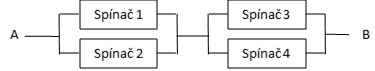
\includegraphics{img.png} \#\#Zadání 1

Problém se dá rozložit na dva podproblémy, kde si první paralelní
spínače označíme jako \alpha a druhé jako \beta. Pak se dá úkol zaspsat
jako:

\[ P(\alpha)=P(S1∨S2)=1-P(\overline{S1}∧\overline{S2})=1-(0.95*0.95)=0.0975
P(\beta)=P(S3∨S4)=1-P(\overline{S3}∧\overline{S4})=1-(0.95*0.95)=0.0975
P(\alpha)*P(\beta)=0.0975*0.0975=0.0095 \]

Výsledná pravděpodobnost, že náhodně zvolený bod čtverce se nachází i v
kruhu, je 0.7853982.

\end{document}
